\chapter{k Selection in Retrieval}
\section{Introduction}
Retrieval-Augmented Generation (RAG) systems enhance language models by grounding responses in externally retrieved documents.A critical challenge in these systems is determining the optimal number of documents (k) to retrieve for a given query.Current approaches fall into three categories: static k selection, which uses a fixed number of retrieved documents; dynamic k selection, which adjusts k based on query  characteristics; and hybrid approaches, which combine both strategies.In this chapter, we first explore methods, highlighting their strengths and limitations We then introduce our novel hybrid dynamic selection algorithm provide detailed description of its methodology and present experimental results that demonstrate the effectiveness of its performance . 
%\section {The Role of k in Retrieval-Augmented Generation}
%The number of retrieved documents (k) is a critical parameter in Retrieval-Augmented Generation (RAG) that has a direct impact on the retrieval and generation phases. Choosing the right k ensures that the system retrieves enough relevant information. 
\section{Defining k: The Number of Retrieved Documents}
the parameter k denotes the number of documents or passages retrieved from an external knowledge base. This retrieval process is managed by the retriever component\cite{pareto2024rag},which identifies the top k relevant documents based on similarity to the query typically using embedding-based search\cite{Rossi_2024} (e.g., dense retrieval with FAISS, BM25, or hybrid methods) Subsequently, these documents are passed to the generator, typically a language model, which synthesizes the final response by integrating the retrieved 
\begin{figure}[h]
	\centering
	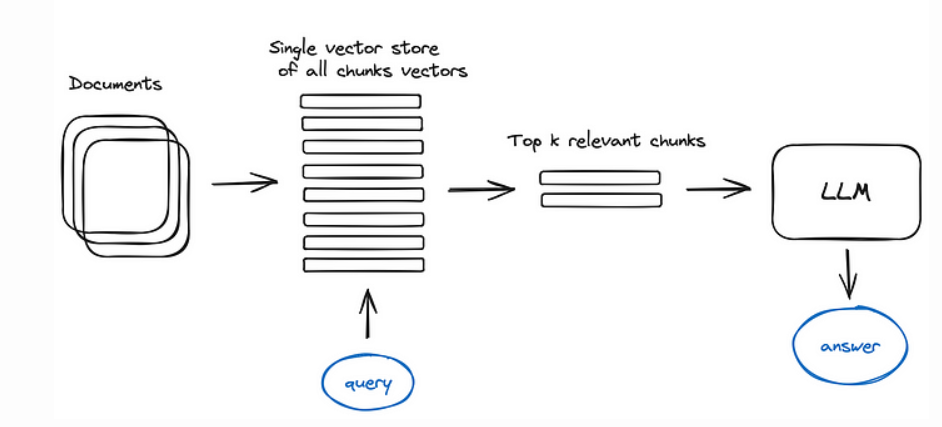
\includegraphics[width=0.9\linewidth]{Figures/topk.png}
	\caption{Basic retrieval}
	\label{rag_retrival.png}
	
\end{figure}
\newline
\section{Impact of k on Retrieval Performance}
The retriever's effectiveness in identifying relevant documents depends on k. Key impacts include :
\subsection{Recall vs. Precision} 
When a user conducts a search query, the outcomes from the database can be grouped into four distinct types based on relevance and retrieval status \cite{geeksforgeeks2022precision}:
\begin{itemize}
	\item {Relevant and Retrieved:} Documents that both address the user’s query and appear in the search results.
	\item {Relevant and Not Retrieved:} Useful documents that answer the query but are not included in the results.
	
	\item {Non-Relevant and Retrieved:} Documents that appear in the results but lack meaningful value for the query.
	 
	\item {Non-Relevant and Not Retrieved:} Irrelevant documents excluded from the results.
\end{itemize}


\textbf{Precision@k}: evaluates the proportion of relevant documents within the top k retrieved results. This metric is particularly valuable in scenarios where the focus is on delivering highly relevant information quickly, rather than ensuring complete coverage such as ,recommendation systems or search engines\cite{deconvoluteai2024metrics}.


\[
\text{Precision@k} = \frac{\text{Number of Relevant Items Retrieved in Top k}}{k}
\]

\textbf{Example}
Suppose we have a dataset of 10 documents. If we retrieve \( k = 4 \) documents and find that 3 of them are relevant to the query:

\begin{itemize}
	\item \textbf{Dataset}: [doc1, doc2, doc3, doc4, doc5, doc6, doc7, doc8, doc9, doc10]
	\item \textbf{Retrieved}: [doc3, doc1, doc7, doc4]
	\item \textbf{Relevant}: [doc1, doc3, doc5, doc8]
\end{itemize}

The Precision@4 score would be:

\[
\text{Precision@4} = \frac{3}{4} = 0.75
\]


\textbf{Recall@k :}evaluates the proportion of relevant documents that are successfully retrieved within the top k results. This metric is particularly important in contexts where ensuring the completeness of information is crucial, such as in medical research or academic tools, where omitting relevant documents could result in incomplete or inaccurate conclusions\cite{deconvoluteai2024metrics}.

\[
\text{Recall@k} = \frac{\text{Number of Relevant Items Retrieved in Top k}}{\text{Total Number of Relevant Items}}
\]
\newline
\textbf{Example}
Consider a dataset of 10 documents. If we retrieve \( k = 4 \) documents and find that 2 of them are relevant, while the total number of relevant documents in the dataset is 4:

\[
\text{Recall@4} = \frac{2}{4} = 0.5
\]


Increasing k typically enhances recall by retrieving more relevant documents but may decrease precision due to the inclusion of irrelevant ones. Conversely, decreasing k can improve precision but at the cost of lower recall. 
\subsection{Retrieval Speed and Computational Cost}
Retrieval speed and computational cost are two important areas where k has a big influence Below is a detailed explanation of how higher k values affect these aspects.

\textbf{Increased Computational Resources:} \\
As the value of k expands, the retrieval system must handle a larger set of documents, leading to higher computational demands. Specifically, the system needs to perform additional operations like ranking, filtering, and similarity scoring to identify the most relevant documents. These tasks become increasingly resource-intensive, particularly in large-scale retrieval settings where the document corpus consists of millions or even billions of entries\cite{manning2008ir}. For instance, retrieving the top  documents (k=80) requires significantly more computational resources compared to retrieving only the top 10 documents (k=5). 

\textbf{Higher Memory Usage:}
As the number of retrieved documents (k) increases ,Storing and processing a larger set of retrieved documents requires more memory This can become a significant bottleneck, especially in environments with constrained memory resources .

For large-scale retrieval tasks, where datasets may contain millions or even billions of documents, the memory demand grows proportionally with 
k. Each retrieved document needs to be stored temporarily, along with its associated metadata, such as embedding vectors, BM25 scores, or other relevance signals. Additionally, sorting and filtering operations further contribute to memory overhead
\subsection{Document Ranking Quality}
Document ranking in information retrieval involves ordering documents by their relevance to a user's query. The objective is to prioritize the most relevant documents at the top of search results, making it easier for users to access useful information quickly. Different models,Vector Space, including Boolean, and Probabilistic models, are used to establish this ranking \cite{enwiki:1262179867}.\\

Increasing the number of retrieved documents,represented as k, may result in the addition of lower-ranked, less relevant documents, potentially diluting the overall quality of the retrieved information. This occurs because of the inherent balance between precision and recall in information retrieval systems.
\begin{figure}[h]
	\centering
	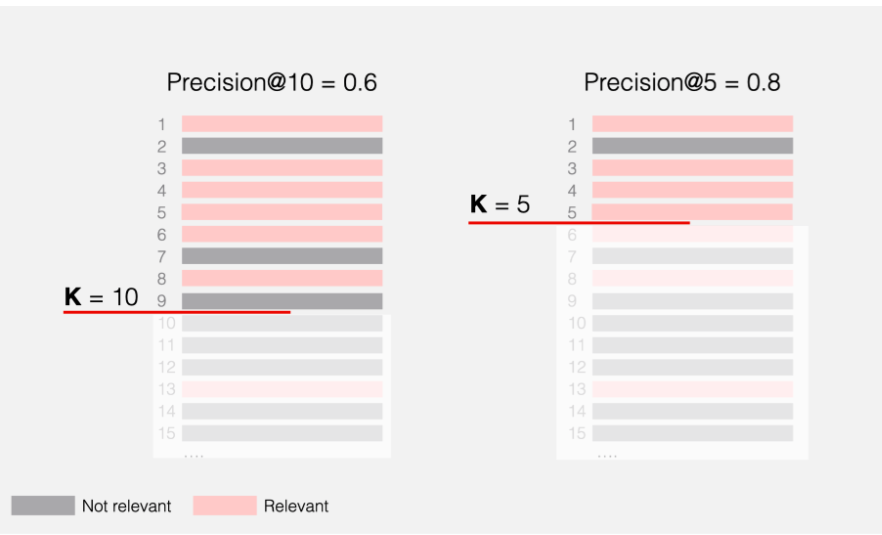
\includegraphics[width=0.7\linewidth]{Figures/precisionR.png}
	\caption{Precision in Document Ranking\cite{evidentlyai2025}}
	\label{precisionR}
	
\end{figure}

\begin{figure}[h]
	\centering
	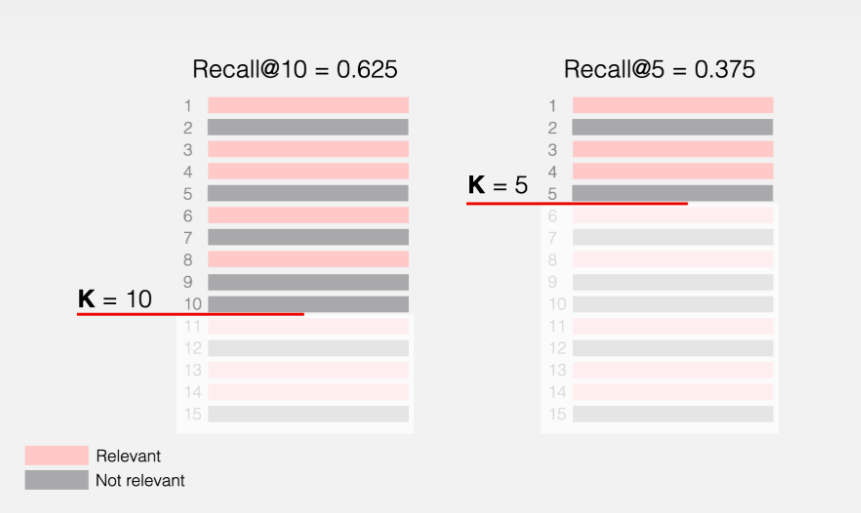
\includegraphics[width=0.7\linewidth]{Figures/recalR.png}
	\caption{Recall in Document Ranking\cite{evidentlyai2025}}
	\label{recalR}
	
\end{figure}
As k grows, recall generally improves since a larger number of relevant documents are likely to be retrieved as shown in Figure \ref{recalR}. However, this often comes at the expense of precision, as the additional documents retrieved may include non-relevant ones,thereby lowering the overall precision as illustrated in Figure \ref{precisionR}. This trade-off is a core principle in evaluating information retrieval systems.

\section{Impact of k on Generation Quality}
The impact of k (the number of retrieved documents or generated candidates) on generation quality is A crucial factor in many machine learning and information retrieval tasks, including text generation, recommendation systems, and search engines . 

\subsection{Trade-off Between Diversity and Relevance} 
Higher k: Increasing k often improves diversity in generated outputs or retrieved documents, as more candidates are considered. However, this can lead to a drop in relevance or quality, as lower-ranked candidates may be less accurate or coherent. \\
Lower k: A smaller k tends to prioritize high-quality, relevant outputs but may lack diversity, leading to repetitive or overly narrow results.

Research shows that the quality of retrieved documents plays a crucial role in the performance of Retrieval-Augmented Generation (RAG) systems. For example, one study demonstrated that the precision of retrieved documents directly affects the factual correctness of the generated responses \cite{salemi2023evaluating}
Additionally, another study revealed that simply increasing the number of documents does not necessarily improve generation quality,especially if the additional documents are not highly relevant\cite{wan2025cognitivealigneddocumentselectionretrievalaugmented}
\subsection {Effect on Text Generation Models}
In text generation tasks, such as machine translation and dialogue systems, The parameter k frequently refers to the beam width in beam search algorithms\cite{freitag-al-onaizan-2017-beam}. Beam search is a heuristic search algorithm that expands the most promising nodes in a graph to maximize the quality of the text that is produced. Adjusting the beam width (k) has significantly impacts how well text generation models function.

As the beam width is increased, the model must process and retain more candidate sequences concurrently, leading to higher computational and memory demands Particularly in real-time applications where latency is crucial, this increase may have an effect on system performance and response time\cite{tensorrt_llm_beam_search}.

\section{Existing Solutions for k Selection}
Selecting an optimalnk plays a crucial role in balancing retrieval effectiveness and generation quality.Over the years, various strategies have been proposed to determine k, ranging from static selection to dynamic and hybrid approaches.
\subsection{Static k Selection}
\subsection{Dynamic k Selection}
\subsection{Hybrid k Selection}
\section{ Proposed Solution}
\subsection{Mixture of Logits-Based k Selection}
\subsection{Algorithm Design}
\subsection{Pseudocode}
\section{ Conclusion }
